\section*{Question 4}
\textcolor{blue}{[Practice with SVD]}


Consider the matrix
\begin{align*}
A = \begin{bmatrix}
-2 & 11\\
-10 & 5\\
\end{bmatrix}    
\end{align*}


\begin{enumerate}
    \item Determine, on paper, a real SVD of $A$ in the form $A = U \Sigma V^T$. The SVD is not unique, so find the one that has the minimal number of minus signs in $U$ and $V$;
    \item List the singular values, left singular vectors, and right singular vectors of $A$. 
    Draw a careful, labeled picture of the unit ball in $\mathbb{R}^2$ and its image under $A$, 
    together with the singular vectors, 
    with the coordinates of their vertices marked;
    \item What are the 1-, 2-, $\infty$-, and Frobenius norms of $A$?
    \item Find $A^{-1}$ not directly, but via the SVD;
    \item Find the eigenvalues $\lambda_1$,  $\lambda_2$ of $A$;
    \item Verify that det $A$ = $\lambda_1\lambda_2$ and $|\det A|=\sigma_1\sigma_2$;
    \item What is the area of the ellipsoid onto which $A$ maps the unit ball in $\mathbb{R}^2$?
\end{enumerate}



\subsection*{Answer}
\subsubsection*{1. SVD Calculation}
\begin{align*}
A &= U \Sigma V^T = \begin{bmatrix}
-2 & 11\\
-10 & 5\\
\end{bmatrix} \\  
\xrightarrow{} 
AA^T &= U \Sigma^2 U^T = \begin{bmatrix}
125 & 75\\
75 & 125
\end{bmatrix} ,\\
A^TA &= V \Sigma^2 V^T = \begin{bmatrix}
    104 & -72\\
    -72 & 146
    \end{bmatrix}
% \xrightarrow{} 
\end{align*}

Conduct eigen decomposition on $AA^T$ and $A^TA$, we get:
\begin{equation*}
    U  = 
    \begin{bmatrix}
        -\sqrt{2}/2 & \sqrt{2}/2\\
        \sqrt{2}/2 & \sqrt{2}/2\\
    \end{bmatrix}, \quad
    \Sigma = 
    \begin{bmatrix}
        5\sqrt{2} & 0\\
        0 & 10\sqrt{2}\\
    \end{bmatrix}, \quad
    V = 
    \begin{bmatrix}
        -4/5 & -3/5\\
        -3/5 & 4/5 
    \end{bmatrix}
\end{equation*}

We adjust $U$ and $V$ so that we get
the minimal number of minus signs,
we turn the sign of $U$'s first column and 
$V$'s first column, and get:

\begin{equation}
    \label{eq:SVD}
    U  = 
    \begin{bmatrix}
        \sqrt{2}/2 & -\sqrt{2}/2\\
        \sqrt{2}/2 & \sqrt{2}/2\\
    \end{bmatrix}, \quad
    \Sigma = 
    \begin{bmatrix}
        5\sqrt{2} & 0\\
        0 & 10\sqrt{2}\\
    \end{bmatrix}, \quad
    V = 
    \begin{bmatrix}
        4/5 & 3/5\\
        -3/5 & 4/5 
    \end{bmatrix}
\end{equation}




\subsubsection*{2. Visualization of SVD.}
From \eqref{eq:SVD} we directly get:
% Singular values: $5\sqrt{2},10\sqrt{2}$; \\
\begin{itemize}
    \item Singular values:
    \begin{equation}
        \label{eq:sigma}
        \sigma_1 = 5\sqrt{2},\quad \sigma_2 = 10\sqrt{2};
    \end{equation}
    \item Left singular vectors:  $[-\sqrt{2}/2, \sqrt{2}/2]^T, [\sqrt{2}/2, \sqrt{2}/2]^T$ ;
    \item Right singular vectors : $[4/5, -3/5]^T, [3/5, 4/5]^T$.
\end{itemize}

% Left singular vectors: $[-\sqrt{2}/2, \sqrt{2}/2]^T, [\sqrt{2}/2, \sqrt{2}/2]^T$ \\
% Right singular vectors : $[4/5, -3/5]^T, [3/5, 4/5]^T$.\\
The unit ball's image under $A$ is show as follow:
\begin{figure}[H]
    \centering
    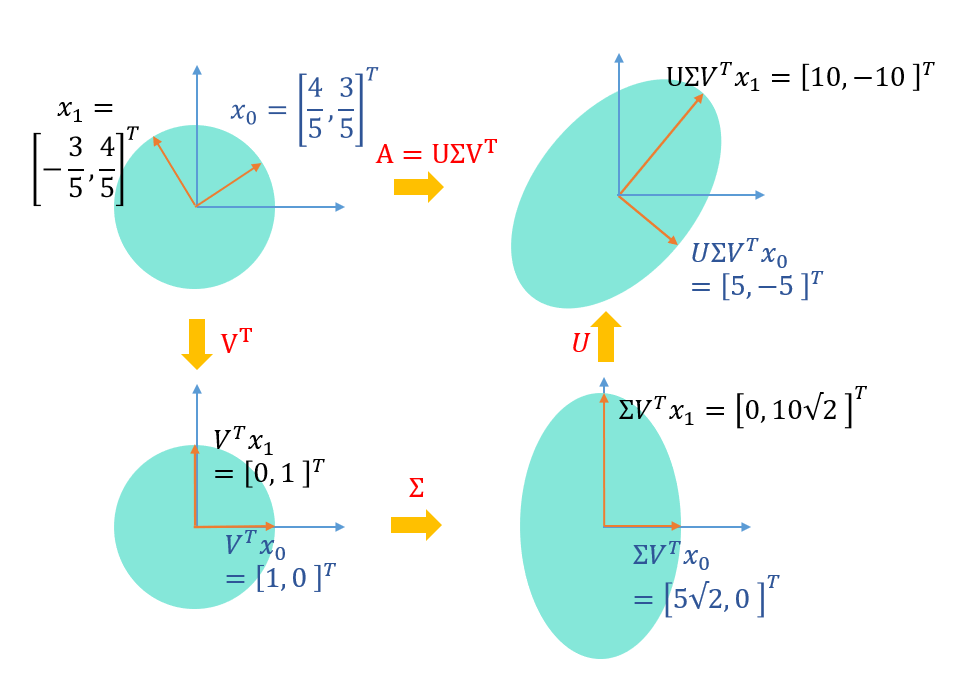
\includegraphics[width=1\textwidth]{SVD_yuhe.png}
    \caption{The unit ball's image under $A$}
    \label{fig:mapping A}
  \end{figure}

\subsubsection*{3. Matrix's Norms}
% 1-, 2-, $\infty$-, and Frobenius norms of $A$
$\|A\|_1 = 28$,\\
$\|A\|_2 = 5\sqrt{10}$,\\
$\|A\|_\infty = 11$,\\
$\|A\|_F = 5\sqrt{10}$

\subsubsection*{4. $A^{-1}$ By SVD \textcolor{red}{[TODO: Check again!]}}
\begin{flalign*}
A^{-1} &= (U \Sigma V^T)^{-1} = {V \Sigma^{-1} U^T} 
    = \begin{bmatrix}
            0.05 & 0.11\\
            -0.1 & -0.02\\
            \end{bmatrix}  &&
\end{flalign*}

\subsubsection*{5. Eigen Values of $A^{-1}$}
The charateristic polynomial of $A$ is:
\begin{equation*}
    p_A(\lambda) = \det(A-\lambda I) = \lambda^2 - 3\lambda + 100,
\end{equation*}
so that we obtain:
%  $\lambda_1 = \dfrac{3+\sqrt{-391}}{2}$ and  $\lambda_2 = \dfrac{3-\sqrt{-391}}{2}$.
\begin{align}
    \label{eq:eigenvalues}
    \left
    \{ \begin{aligned}
        \lambda_1 &= \dfrac{3+\sqrt{-391}}{2} \\ \lambda_2 &= \dfrac{3-\sqrt{-391}}{2}
    \end{aligned}
    \right.
\end{align}

\subsubsection*{6. Relationship of Eigen Values and Matrixs' Determinant and Trace}
From \eqref{eq:eigenvalues} and \eqref{eq:sigma}, we get:
\begin{align*}
    % \label{eq:eigenvalues}
    \left
    \{ \begin{aligned}
        \lambda_1\lambda_2 &= 100 = \det A \\ 
        \sigma_1\sigma_2   &= 100 = |\det A|\\
    \end{aligned}
    \right.
\end{align*}




\subsubsection*{7. Ellipsoid Mapped $A^{-1}$}
Figure \ref{fig:mapping A} has been shown in sub-question 2,
now we describe the mapped-to ellipsoid analytically:
\\
The unit ball before mapped by $A$ is :
\begin{equation*}
    \{\ (x,y) \ |\ [x,y]     
                    \begin{bmatrix}
                        1 & 0\\
                        0 & 1\\
                    \end{bmatrix}
                    \begin{bmatrix}
                        x\\
                        y\\
                    \end{bmatrix}   \leq 1  
    \}.
\end{equation*}
\\
After being mapped by $A$, the set of points comes to:
\begin{equation*}
    \{\ (x,y) \ |\ ([x,y]A^T)
                    \begin{bmatrix}
                        1 & 0\\
                        0 & 1\\
                    \end{bmatrix}
                    (A
                    \begin{bmatrix}
                        x\\
                        y\\
                    \end{bmatrix})  \leq 1  
    \},
\end{equation*}
which can be written as:
\begin{equation}
    \label{eq:analytical_epi}
    \{\ (x,y) \ |\ [x,y]A^TA
                    \begin{bmatrix}
                        x\\
                        y\\
                    \end{bmatrix}  \leq 1  
    \}.
\end{equation}
Equation \eqref{eq:analytical_epi} is just the analytical solution
of obtain ellipsoid.
